\section{Introduction}
Natural and man-made disasters causing structural damage to inhabited buildings are an ever-present danger. As time-to-rescue is one of the most important factors that determines the victims` survivability, it is of highest importance for the rescue responders to reach victims as fast as possible to provide them with medical attention or extraction. Planning and executing optimal paths through buildings is, however, difficult as structural damage makes floor plans outdated. Furthermore, structural weaknesses, as well as hazardous environments, can make localized regions or whole areas inaccessible. While trained responders can use their knowledge and intuition to spot these hazards, it is paramount that the Incident Commander (IC), who has global information about the building, can analyze the information and coordinate the rescue responders. To design an effective system amplifying human decision-making, it is vital to consider how decisions in dynamic unpredictable situations are made~\cite{Lundberg2012}. The system can then be designed to amplify the ability to plan based on experience, to increase quality of control, and to support decision-making not only with regard to expected decisions, but also regarding unexpected developments.

There are well defined protocols in place to describe the actions taken during an Urban Search~\&~Rescue (USAR) event. The Federal Emergency Management Agency describes five steps that are performed by the rescue team. During an assessment step, two dimensional maps of the collapsed building are hand-drawn based on the descriptions of rescue responders, who are moving within the building searching for victims (see Figure~\ref{fig:workflow:sota}). In this exploration phase, they might stumble into hazardous areas, such as gas leaks, that endanger the rescuer`s life. Even though the guidelines require these sketches to include a cross section of the building, a drawing of an unstructured three dimensional building is inaccurate and ineffective to construct a correct mental model, yet this is the currently employed technique.

In recent years, technological developments made it possible to use ground-based unmanned vehicles to perform the initial exploration. These robots can be deployed into the building and are equipped with sensors that can detect victims, gather information about potentially hazardous environments, and perform detailed scans of rooms to create a three-dimensional point cloud data of the building`s interior. These unstructured point clouds are collated and co-registered to produce a consistent map of the building. Using simultaneous localization and mapping algorithms~\cite{Dissanayake01asolution, Ziparo459917}, this map can be used to navigate the robots through buildings while exploring accessible areas. After the map has been acquired, the \IC\ can analyze the collected data and plan viable access paths for the rescue responders that enter the building to reach certain \emph{Points of Interests} (POIs). In most cases, these POIs are potential locations of victims, but they can also be other critical areas that need to be reached and analyzed.

In this paper, we propose a visualization system that uses the acquired and annotated map during USAR missions to support access path planning. The system preprocesses the point cloud data to create an interactive three-dimensional rendering that is tailored to increase the commander`s spatial awareness of the internal structure and further supports the analysis and the planning of viable access paths. The awareness is paramount in detecting the location of unreachable areas, so called voids, a prime location where victims might be trapped. The gained information is used to instruct rescue responders to reach several POIs and the \IC\ can annotate the visualization with new real-time information that he receives from the on-site rescue responders, thus shifting the decision making process from being opportunistic to being strategical. Based on the available information, our system computes an ensemble of possible access paths from the entry point to the POIs, where each path is based on varying risk factors, for example overall distance, closest distance to a hazard, or the structural stability. Uncertainty in the data and a priori unknown information make it infeasible to employ fully automatic algorithms to detect the globally optimal path. Our system supports the \IC\ in the process of analyzing and comparing all available paths at once to reach a conclusion which minimizes the rescuer`s travel time and danger. In our system, we combine robot-based data acquisition and automated path planning with newly added information and the decision-making of the expert user with the goal to increase the probability of saving the victims` lives.

Combining expertise in visualization, cognitive systems engineering, rescue robotics, and through discussions with the domain experts, we determined a set of requirements that must be fulfilled to make our system useful for the \IC . We employed theories from sense-making and decision-making (Section~\ref{sec:theory}) to guide the design of our system to fully support the \IC\ in his tasks. The visualization components are arranged to comply with this theory. From the analysis we derive the following requirements:
\begin{description}
\item[R1] The system must increase the \IC `s spatial awareness and allow for interactive exploration of the collapsed structure
\item[R2] The system must enable the \IC\ to interactively annotate the acquired data to react to changing circumstances
\item[R3] The \IC\ must be able to inspect the classes of optimal paths and be able to compare these
\item[R4] The system must provide the tools to select a globally optimal path
\end{description}

\begin{figure}
	\centering
	\framebox[0.65\columnwidth][c]{
	    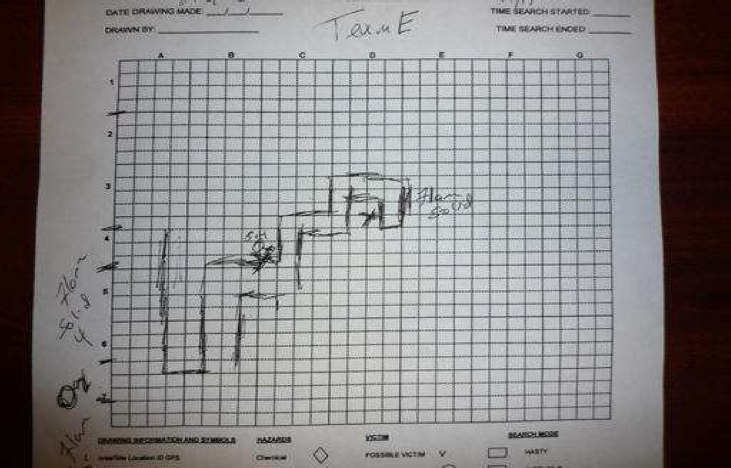
\includegraphics[width=0.65\columnwidth]{figures/map-drawing.jpg}
	}
	\caption{The currently employed workflow requires the \IC\ to draw a two-dimensional map by hand for orientation.}
	\label{fig:workflow:sota}
\end{figure}
